\documentclass[12pt]{article}
\usepackage[utf8]{inputenc}
\usepackage{amsmath, amssymb, amsthm}
\usepackage{geometry}
\usepackage{graphicx}
\usepackage{tikz}
\usepackage{bm}
\usetikzlibrary{shapes,arrows,positioning}
\usepackage{hyperref}
\usepackage{tocloft}
\usepackage{xcolor}
\usepackage{enumitem}
\usepackage{tcolorbox}
\usepackage{enumitem}
\usepackage{booktabs}

% Page layout
\geometry{a4paper, margin=1in}

% Custom colors
\definecolor{harvardcrimson}{RGB}{165, 28, 48}
\definecolor{lectureblue}{RGB}{0, 76, 151}
\definecolor{bookgreen}{RGB}{0, 102, 51}

% Custom commands
\newcommand{\lecture}[1]{\section*{Lecture #1 \hfill \normalsize\textcolor{gray}{Stat 110}}%
\addcontentsline{toc}{section}{Lecture #1}}
\newcommand{\bookref}[1]{\textcolor{bookgreen}{\textbf{[Blitzstein #1]}}}
\newcommand{\important}[1]{\textcolor{harvardcrimson}{\textbf{#1}}}
\newcommand{\definition}[1]{\begin{tcolorbox}[colback=blue!5!white,colframe=lectureblue,title=Definition] #1 \end{tcolorbox}}
\newcommand{\theorem}[1]{\begin{tcolorbox}[colback=green!5!white,colframe=bookgreen,title=Theorem] #1 \end{tcolorbox}}
\newcommand{\example}[1]{\begin{tcolorbox}[colback=yellow!5!white,colframe=orange!50!black,title=Example] #1 \end{tcolorbox}}
\newcommand{\note}[1]{\begin{tcolorbox}[colback=red!5!white,colframe=red!70!black,title=Note] #1 \end{tcolorbox}}
\newcommand{\story}[1]{\begin{tcolorbox}[colback=purple!5!white,colframe=purple!70!black,title=Story] #1 \end{tcolorbox}}

\newcommand{\Bin}{\text{Bin}}
\newcommand{\Bern}{\text{Bern}}
\newcommand{\HGeom}{\text{HGeom}}


% Header with course info
\usepackage{fancyhdr}
\pagestyle{fancy}
\fancyhead[L]{\small Stat 101: Introduction to Probability}
\fancyhead[C]{\small Lecture Notes}
\fancyhead[R]{\small Harvard University}
\fancyfoot[C]{\thepage}

\title{\textbf{Stat 110 Lecture Notes}\\Harvard Statistics 110\\by\\Pedro N. Jorge}
\author{Based on Blitzstein's lectures and book "Introduction to Probability"}
\date{Fall 2023}

\begin{document}

\maketitle

\tableofcontents

\newpage
\lecture{1: Probability and Counting}
\textbf{Key Topics:} Sample spaces, events, naive probability definition, counting

\subsection*{Lecture Summary}
\begin{itemize}
\item Definition of sample spaces and events
\item Introduction to probability in a naive way
\item Basic principles of counting
\end{itemize}

\subsection*{Core Concepts}

\definition{\textbf{Sample Space and Event} (\bookref{Ch. 1.2})\\
The \textbf{sample space}, often denoted by $\Omega$ or $S$, of an experiment is the set of all possible outcomes of the experiment. An \textbf{event} $A$ is a subset of the sample space S, and we say that A \textit{occurred} if the actual outcome is in A.}

\definition{\textbf{Naive definition of Probability} (\bookref{Ch. 2.1})\\
$P(A) = \frac{|A|}{|S|} =\frac{\# \text{ favorable outcomes}}{\# \text{ possible outcomes}}$ \\
Assume all outcomes are equally likely and the sample space is finite.}

\definition{\textbf{Binomial Coefficient} (\bookref{Ch. 1.2})\\
The \textbf{binomial coefficient} $\binom{n}{k}$, read as "$n$ choose $k$", is the number of subsets of size $k$ for a set of size $n$. We are counting the number of ways to choose $k$ objects out of $n$, \textit{without replacement and without order}.
}
\subsection*{Counting}

\theorem{\textbf{Multiplication Rule} (\bookref{Ch. 1.4.1})\\
Consider a compound experiment consisting of two sub-experiments, Experiment A and Experiment B. Suppose that Experiment A has $a$ possible outcomes, and for each of those outcomes Experiment B has $b$ possible outcomes. Then the compound experiment has $ab$ possible outcomes.}
\note{It is often easier to think about the experiments as being in chronological order, but there is no requirement in the multiplication rule that Experiment A has to be performed before Experiment B.}

\theorem{\textbf{Sampling with replacement} (\bookref{Ch. 1.4.8})\\
Consider $n$ objects and making $k$ choices from them, one at a time \textit{with replacement} (i.e., choosing a certain object does not preclude it from being chosen again). Then there are $n^k$ possible outcomes (where order matters, in the sense that, e.g., choosing object 3 and then object 7 is counted as a different outcome than choosing object 7 and then object 3.)}

\theorem{\textbf{Sampling without replacement} (\bookref{Ch. 1.4.7})\\
Consider $n$ objects and making $k$ choices from them, one at a time \textit{without replacement} (i.e., choosing a certain object precludes it from being chosen again). Then there are $n(n - 1)\cdots(n - k + 1)$ possible outcomes for $1 \le k \le n$, and 0 possibilities for $k > n$ (where order matters). By convention, $n(n - 1)\cdots(n - k + 1) = n$ for $k = 1$. \\
This result also follows directly from the multiplication rule: each sampled ball is again a sub-experiment, and the number of possible outcomes decreases by 1 each time. Note that for sampling $k$ out of $n$ objects without replacement, we need $k \le n$, whereas in sampling with replacement the objects are inexhaustible.}

\note{\textbf{Labelling objects}\\
Drawing a sample from a population is a very fundamental concept in statistics. It is important to think of the objects or people in the population as named or labeled. For example, if there are $n$ balls in a jar, we can imagine that they have labels from 1 to $n$, even if the balls look the same to the human eye. In the birthday problem, we can give each person an ID (identification) number, rather than thinking of the people as indistinguishable particles or a faceless mob.}

In many counting problems, it is not easy to directly count each possibility once and only once. If, however, we are able to count each possibility exactly $c$ times for some $c$, then we can adjust by dividing by $c$. For example, if we have exactly double-counted each possibility, we can divide by 2 to get the correct count. We call this \textit{adjusting for overcounting}.

\example{Consider a group of four people
\begin{enumerate}[label=(\alph*)]
    \item How many ways are there to choose a two-person committee?
    \item How many ways are there to break the people into two teams of two?
\end{enumerate}
(a) By the multiplication rule, there are 4 ways to choose the first person on the committee and 3 ways to choose the second person on the committee, but this counts each possibility twice, since picking 1 and 2 to be on the committee is the same as picking 2 and 1 to be on the committee. Since we have overcounted by a factor of 2, the number of possibilities is $(4 \cdot 3) / 2 = 6$.\\
(b) Using (a) we see that there are 6 ways to choose one team. This overcounts by a factor of 2, since picking 1 and 2 to be a team is equivalent to picking 3 and 4 to be a team. So the answer is $6/2 = 3$.
}

\subsection*{Sample Table}
\begin{center}
\begin{tabular}{c|cc}
 & \textbf{Order Matters} & \textbf{Order Doesn't Matter} \\
\hline
\textbf{Replace} & $n^k$ & $\binom{n + k - 1}{k}$\\[0.5em]
\hline
\textbf{Don't Replace} & $n(n-1)\cdots(n-k-1)$ & $\binom{n}{k}$ \\[0.5em]
\end{tabular}
\end{center}

The top right entry will be explained in Lecture 2. The other entries simply come from the multiplication rule and are intuitive.
\newpage
\lecture{2: Story Proofs, Axioms of Probability}
\textbf{Key Topics:} Story proofs, general definiton of probability

\subsection*{Lecture Summary}
\begin{itemize}
    \item Revisit sampling with replacement and without order
    \item Story proofs
    \item General definition of probability
\end{itemize}

\subsection*{Core Concepts}
\definition{\textbf{General definition of probability} (\bookref{Ch. 1.6})\\
A \textit{probability space} consists of a sample space $S$ and a probability function $P$ which takes an event $A \subseteq S$ as input and returns $P(A) \in [ 0, 1]$ as output. The function $P$ must satisfy the following axioms:
\begin{enumerate}[label=(\arabic*)]
    \item $P(\emptyset) = 0$, $P(S) = 1$.
    \item If $A_1, A_2, \dots$ are disjoint events, then
$$
P\left( \bigcup^\infty_{j=1} A_j \right) = \sum^\infty_{j=1} P(A_j).
$$
\end{enumerate}
}
\subsection*{Sampling with replacement and without order}

Pick $k$ times from a set of $n$ objects, where order doesn't matter. The result is $\binom{n+k-1}{k}$ ways. Let's see why by reframing our problem.

Equivalently, we want to know how many ways to put $k$ indistinguishable particles into $n$ distinguishable boxes. We can represent it graphically using '$*$' to represent particles and '$|$' to represent boxes ($n=4$ and $k=6$):
\begin{equation*}
    ***||**|*
\end{equation*}
There must be $k$ $*$'s and $n-1$ $|$'s. So, in total there are $n+k-1$ symbols and we just need to choose the position of the $*$'s. Therefore, the result is $\binom{n+k-1}{k}$.

\subsection*{Story Proofs (proof by interpretation)}

A \textbf{story proof} is a proof by interpretation. For counting problems, this often means counting the same thing in two different ways, rather than doing tedious algebra. A story proof often avoids messy calculations and goes further than an algebraic proof toward \textit{explaining} why the result is true. The word “story” has several meanings, some more mathematical than others, but a story proof (in the sense in which we’re using the term) is a fully valid mathematical proof.

\example{$$n\binom{n-1}{k-1} = k\binom{n}{k}$$
Pick $k$ people out of $n$, with one designated as President. There is two different approaches to take:
\begin{itemize}
    \item First select who is in the club $\binom{n}{k}$, and one of those $k$ members must be elected President: $k\cdot \binom{n}{k}$
    \item First choose the President, and then, we need $k-1$ people to be in the club, out of the remaining $n-1$: $n \cdot \binom{n-1}{k-1}$
\end{itemize}
}

\example{\textbf{Vandermonde's identity}\\
$$\binom{m+n}{k} = \sum^k_{j=0} \binom{m}{j}\binom{n}{k-j}$$
Pick $k$ people out of two distinct groups of $m$ and $n$ people, respectively $G_m$ and $G_n$. This means that if we pick $j$ people from $G_m$, we pick $k-j$ people from $G_n$, since we need to pick $k$ in total. Therefore, we can look at every case, going from picking 0 people from $G_m$ to picking all $k$.
}
\newpage
\lecture{3: Birthday Problem, Properties of Probability}
\textbf{Key Topics:} Birthday problem, properties of probability, inclusion-exclusion

\subsection*{Lecture Summary}
\begin{itemize}
    \item Birthday problem that defies intuition
    \item Properties of probability given the axioms
    \item Inclusion-exclusion theorem and application
\end{itemize}

\subsection*{Birthday Problem}

There are $k$ people in a room. Assume each person’s birthday is equally likely to be any of the 365 days of the year (we exclude February 29), and that people’s birthdays are independent (we will define independence formally later, but intuitively it means that knowing some people’s birthdays gives us no information about other people’s birthdays; this would not hold if, e.g., we knew that two of the people were twins). What is the probability that at least one pair of people in the group have the same birthday?

If $k > 365$, by the pigeonhole principle, the probability is 1. Let $k\le 365$.

\begin{align*}
    &P(\text{no match}) = \frac{365\cdot364\cdots(365-k+1)}{365^k} \\
    \implies &P(match) \approx 
    \begin{cases}
        50.7 \%, & \text{if } k=23 \\
        97\%, & \text{if } k=50 \\
        99.99\%, & \text{if } k=100
    \end{cases}
\end{align*}

It’s surprising that even with a much smaller number of people it’s overwhelmingly likely that there is a birthday match. For a quick intuition into why it should not be so surprising, note that with 23 people there are $\binom{23}{2} = 253$ \textit{pairs} of people, any of which could be a birthday match.

\subsection*{Properties of Probability}

\theorem{\textbf{Properties of Probability} (\bookref{Ch. 1.6})\\
Probability has the following properties, for any events $A$ and $B$.
\begin{enumerate}[label=\arabic*.]
    \item $P(A^c) = 1 - P(A)$.
    \item If $A \subseteq B$, then $P(A) \le P(B)$.
    \item $P(A\cup B) = P(A) + P(B) - P(A\cap B)$.
\end{enumerate}
\textit{Proof.}
\begin{enumerate}[label=\arabic*.]
    \item Since $A$ and $A^c$ are disjoint and their union is $S$,
    $$
    1=P(S)=P(A\cup A^c) = P(A)+P(A^c)
    $$
    \item If $A \subseteq B$, then $B = A \cup (B\cap A^c)$, where $A$ and $(B\cap A^c)$ disjoint.
    $$
    P(B) = P(A) + P (B \cap A^c) \ge P(A)
    $$
    \item $P(A\cup B) = P(A \cup (B \cap A^c)) = P(A) + P(B \cap A^c)$. It suffices to show that $P(B \cap A^c) = P(B) - P(A\cap B)$, but we know that $B = (A \cap B) \cup (A^c \cap B)$ which are disjoint.
\end{enumerate}

}

The third property is a special case of \textit{inclusion-exclusion}, a formula for finding the probability of a union of events when the events are not necessarily disjoint. For three events, inclusion-exclusion says
\begin{align}
    P(A\cup B \cup C) = &P(A) + P(B) + P(C)\\
    &-P(A\cap B) - P(A \cap C) - P(B \cap C)\\
    &+P(A\cap B\cap C)
\end{align}

For intuition consider this Venn Diagram:
\begin{center}
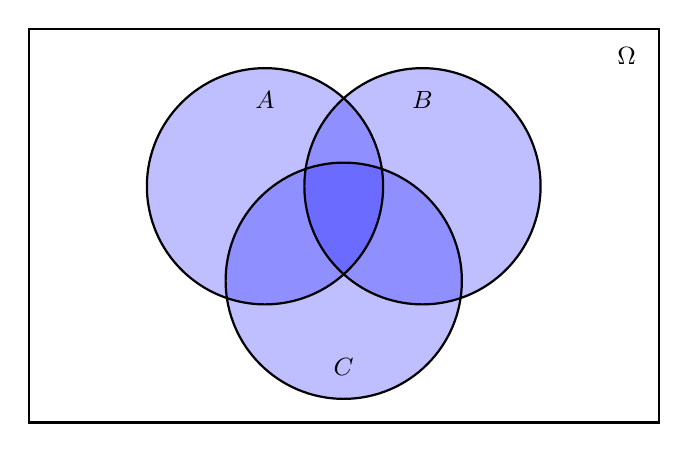
\begin{tikzpicture}[font=\small]
  % Parameters
  \def\W{8}   % rectangle width
  \def\H{5}   % rectangle height
  \def\r{1.5} % circle radius

  % Rectangle (sample space)
  \draw[thick] (0,0) rectangle (\W,\H) node[pos=0.98,below left] {$\Omega$};

  % Clip everything to the rectangle so circles stay inside
  \begin{scope}
    \clip (0,0) rectangle (\W,\H);

    % Fill the union by filling each circle with same color and opacity
    \fill[blue,opacity=0.25] (3.0,3.0) circle (\r); % A
    \fill[blue,opacity=0.25] (5.0,3.0) circle (\r); % B
    \fill[blue,opacity=0.25] (4.0,1.8) circle (\r); % C
  \end{scope}

  % Draw circle outlines and labels
  \draw[thick] (3.0,3.0) circle (\r) node[yshift=1.1cm] {$A$};
  \draw[thick] (5.0,3.0) circle (\r) node[yshift=1.1cm] {$B$};
  \draw[thick] (4.0,1.8) circle (\r) node[yshift=-1.1cm] {$C$};

  % Title / probability text
  %\node at (4,-0.5) {$P(A\cup B\cup C)$};

\end{tikzpicture}
\end{center}
To get the total area of the shaded region $A \cup B \cup C$, we start by adding the areas of the three circles, $P(A) + P(B) + P(C)$. The three football-shaped regions have each been counted twice, so we then subtract $P(A \cap B) + P(A \cap C) + P(B \cap C)$. Finally, the region in the center has been added three times and subtracted three times, so in order to count it exactly once, we must add it back again. This ensures that each region of the diagram has been counted once and exactly once

Now we can write inclusion-exclusion for $n$ events.

\theorem{\textbf{Inclusion-exclusion} (\bookref{Ch. 1.6})\\
For any events $A_1, \dots, A_n$,
\begin{align*}
    P\left( \bigcup^n_{i=1} A_i\right) = \sum_i P(A_i) - \sum_{i < j}P(A_i \cap A_j) + \sum_{i < j< k} P(A_i \cap A_j \cap A_k) -\dots\\
    +(-1)^{n+1} P(A_1 \cap \dots \cap A_n).
\end{align*}
}

This formula can be proven by induction using just the axioms, but instead we’ll present a shorter proof later on after introducing some additional tools. The rationale behind the alternating addition and subtraction in the general formula is analogous to the special cases we’ve already considered.

The next example, \textit{de Montmort’s matching problem}, is a famous application of inclusion-exclusion. Pierre Rémond de Montmort was a French mathematician who studied probability in the context of gambling and wrote a treatise devoted to the analysis of various card games. He posed the following problem in 1708, based on a card game called Treize.

\example{\textbf{de Montmort's matching problem}\\
Consider a well-shuffled deck of $n$ cards, labeled 1 through $n$. You flip over the cards one by one, saying the numbers 1 through $n$ as you do so. You win the game if, at some point, the number you say aloud is the same as the number on the card being flipped over (for example, if the 7th card in the deck has the label 7). What is the probability of winning?

Let $A_i$ be the event that the $i$th card in the deck has the number $i$ written on it. We are interested in the probability of the union $A_1 \cup \cdots \cup A_n$: as long as at least one of the cards has a number matching its position in the deck, you will win the game. First,
$$
P(A_i) = \frac{1}{n}.
$$
By symmetry: the card numbered $i$ is equally likely to be in any of the $n$ positions in the deck, so it has probability $1/n$ of being in the $i$th spot. Second,
$$
P(A_i \cap A_j) = \frac{(n-2)!}{n!} = \frac{1}{n(n-1)},
$$
since we require the cards numbered $i$ and $j$ to be in the $i$th and $j$th spots in the deck and allow the remaining $n-2$ cards to be in any order, so $(n-2)!$ out of $n!$ possibilities are favorable. Similarly,
$$
P(A_i \cap A_j \cap A_k) = \frac{1}{n(n-1)(n-2)}.
$$
In the inclusion-exclusion formula, there are $n$ terms involving one event, $\binom{n}{2}$ terms involving two events, $\binom{n}{3}$ terms involving three events, and so forth. By the symmetry of the problem, all $n$ terms of the form $P(A_i)$ are equal, all $\binom{n}{2}$ terms of the form $P(A_i \cap A_j)$ are equal, and the whole expression simplifies considerably:
\begin{align*}
    P\left( \bigcup^n_{i=1} A_i\right) &= n\cdot \frac{1}{n} - \binom{n}{2} \cdot \frac{1}{n(n-1)} + \binom{n}{3} \cdot \frac{1}{n(n-1)(n-2)} - \cdots + (-1)^{n+1} \cdot \frac{1}{n!}\\
    &= 1 - \frac{1}{2!} + \frac{1}{3!} - \cdots + (-1)^{n+1} \cdot \frac{1}{n!}\\
    &\approx 1 - \frac{1}{e}
\end{align*}
}
\newpage
\lecture{4: Conditional Probability}
\textbf{Key Topics:} Independent events, conditional probability definition, Bayes' rule

\subsection*{Lecture Summary}
\begin{itemize}
    \item Definition of independent events
    \item Newton-Pepys problem
    \item Definition of conditional probability
    \item Conditional probability theorems
\end{itemize}

\subsection*{Core Concepts}

\definition{\textbf{Independence of two events} (\bookref{Ch. 2.5})\\
Events $A$ and $B$ are \textit{independent} if
$$
P(A \cap B) = P(A)P(B).
$$
If $P(A) > 0$ and $P(B) > 0$, then this is equivalent to
$$
P(A|B)  =P(A),
$$
and also equivalent to $P(B|A) = P(B)$.
}
\note{Independence is completely different from disjointness. If $A$ and $B$ are disjoint, then $P(A\cap B) = 0$, so disjoint events can be independent only if $P(A) = 0$ or $P(B) = 0$. Knowing that $A$ occurs tells us that $B$ definitely did not occur, so $A$ clearly conveys information about $B$, meaning the two events are not independent (except if A or B already has zero probability).}

\definition{\textbf{Independence of three events} (\bookref{Ch. 2.5})\\
Events $A$, $B$, and $C$ are said to be \textit{independent} if all of the following equations hold:
\begin{align*}
    P(A \cap B) &= P(A)P(B),\\
    P(A \cap C) &= P(A)P(C),\\
    P(B \cap C) &= P(B)P(C),\\
    P(A \cap B \cap C) &= P(A)P(B)P(C).
\end{align*}
If the first three conditions hold, we say that A, B, and C are \textit{pairwise independent}. Pairwise independence does \textit{not} imply independence: it is possible that just learning about $A$ or just learning about $B$ is of no use in predicting whether $C$ occurred, but learning that both $A$ and $B$ occurred could still be highly relevant for $C$. Here
is a simple example of this distinction.
}

\definition{\textbf{Independence of many events} (\bookref{Ch. 2.5})\\
For $n$ events $A_1, A_2, \dots, A_n$ to be \textit{independent}, we require any pair to satisfy $P(A_i \cap A_j) = P(A_i)P(A_j)$ (for $i \neq j$), any triplet to satisfy $P(A_i \cap A_j \cap A_k) = P(A_i)P(A_j)P(A_k) $ (for $i$, $j$, $k$ distinct), and similarly for all quadruplets, quintuplets, and so on. This can quickly become unwieldy, but later we will discuss other ways to think about independence. For infinitely many events, we say that they are independent if every finite subset of the events is independent.
}

\definition{\textbf{Conditional probability} (\bookref{Ch. 2.2})\\
If $A$ and $B$ are events with $P(B) > 0$, then the \textit{conditional probability} of $A$ given $B$, denoted by $P(A|B)$, is defined as
$$
P(A|B) = \frac{P(A \cap B)}{P(B)}.
$$
Here $A$ is the event whose uncertainty we want to update, and $B$ is the evidence we observe (or want to treat as given). We call $P(A)$ the \textit{prior} probability of A and $P(A|B)$ the \textit{posterior} probability of $A$ (“prior” means before updating based on the evidence, and “posterior” means after updating based on the evidence).
For any event $A$, $P(A|A) = P(A \cap A) / P(A) = 1$. Upon observing that $A$ has occurred, our updated probability for $A$ is 1. If this weren’t the case, we would demand a new definition of conditional probability!
}

\subsection*{Conditional probability}

\theorem{\textbf{Probability of the intersection of two events} (\bookref{Ch. 2.3})\\
For any events $A$ and $B$ with positive probabilities,
$$
P(A \cap B) = P(B)P(A|B) = P(A)P(B|A).
$$
This follows from taking the definition of $P(A|B)$ and multiplying both sides by $P(B)$, and then taking the definition of $P(B|A)$ and multiplying both sides by $P(A)$. We will see that the theorem is in fact very useful, since it often turns out to be possible to find conditional probabilities without going back to the definition.
}

\theorem{\textbf{Probability of the intersection of $\bm{n}$ events} (\bookref{Ch. 2.3})\\
For any events $A_1, \dots, A_n$ with $P(A_1, A_2, \dots, A_{n-1}) > 0$,
$$
P(A_1, A_2, \dots, A_n) = P(A_1)P(A_2|A_1)P(A_3|A_1, A_2) \cdots P(A_n|A_1, \dots, A_{n-1}).
$$
In fact, this is $n!$ theorems in one, since we can permute $A_1, \dots, A_n$ however we want without affecting the left-hand side. Often the right-hand side will be much easier to compute for some orderings than for others. For example,
$$
P(A_1, A_2, A_3) = P(A_1)P(A_2 |A_1)P(A_3|A_1,A_2) = P(A_2)P(A_3|A_2)P(A_1|A_2,A_3),
$$
and there are 4 other expansions of this form too. It often takes practice and thought to be able to know which ordering to use.
}

\theorem{\textbf{Bayes' Rule} (\bookref{Ch. 2.3})\\
$$
P(A|B) = \frac{P(B|A)P(A)}{P(B)}.
$$
This follows immediately from the previous theorems, which in turn follow immediately from the definition of conditional probability. Yet Bayes’ rule has important implications and applications in probability and statistics, since it is so often necessary to find conditional probabilities, and often $P(B|A)$ is much easier to find directly than $P(A|B)$ (or vice versa).
}
\newpage
\lecture{5: Conditioning Continued, Law of Total Probability}
\textbf{Key Topics:} Law of total probability, conditional independent events

\subsection*{Lecture Summary}
\begin{itemize}
    \item Law of total probability (LOTP)
    \item Definition of conditional independence
    \item Reinforce the difference between conditional independence and unconditional independence
\end{itemize}

\subsection*{Core Concepts}

\definition{\textbf{Conditional Independece} (\bookref{Ch. 2.5})\\
Events $A$ and $B$ are said to be conditionally independent given $E$ if $P(A \cap B|E) = P(A|E)P(B|E)$.
}

\note{
It is easy to make terrible blunders stemming from confusing independence and conditional independence. Two events can be conditionally independent given $E$, but not independent given $E^c$. Two events can be conditionally independent given $E$, but not independent. Two events can be independent, but not conditionally
independent given $E$.

In particular, $P(A, B) = P(A)P(B)$ does not imply $P(A, B|E) = P(A|E)P(B|E)$; we can’t just insert “given $E$” everywhere, as we did in going from LOTP to LOTP with extra conditioning. This is because LOTP always holds (it is a consequence of the axioms of probability), whereas $P(A, B)$ may or may not equal $P(A)P(B)$, depending on what $A$ and $B$ are.
}

The next few examples illustrate these distinctions. Great care is needed in working with conditional probabilities and conditional independence!

\example{\textbf{Conditional independence given $\bm{E}$ vs. given $\bm{E^c}$}\\
Suppose there are two types of classes: good classes and bad classes. In good classes, if you work hard, you are very likely to get an A. In bad classes, the professor randomly assigns grades to students regardless of their effort. Let $G$ be the event that a class is good, $W$ be the event that you work hard, and $A$ be the event that you receive an A. Then $W$ and $A$ are conditionally independent given $G^c$, but they are not conditionally independent given $G$.
}

\example{\textbf{Conditional independence doesn’t imply independence}\\
Suppose we have chosen either a fair coin or a biased coin with probability 3/4 of Heads, but we do not know which one we have chosen. We flip the coin a number of times. Conditional on choosing
the fair coin, the coin tosses are independent, with each toss having probability 1/2 of Heads. Similarly, conditional on choosing the biased coin, the tosses are independent, each with probability 3/4 of Heads.\\

However, the coin tosses are not unconditionally independent, because if we don’t know which coin we’ve chosen, then observing the sequence of tosses gives us information about whether we have the fair coin or the biased coin in our hand. This in turn helps us to predict the outcomes of future tosses from the same coin.\\

To state this formally, let $F$ be the event that we’ve chosen the fair coin, and let $A_1$ and $A_2$ be the events that the first and second coin tosses land Heads. Conditional on $F$, $A_1$ and $A_2$ are independent, but $A_1$ and $A_2$ are not unconditionally independent because $A_1$ provides information about $A_2$.
}

\example{\textbf{Independence doesn’t imply conditional independence}\\
My friends Alice and Bob are the only two people who ever call me on the phone. Each day, they decide independently whether to call me that day. Let $A$ be the event that Alice calls me next Friday and $B$ be the event that Bob calls me next Friday. Assume $A$ and $B$ are unconditionally independent with $P(A) > 0$ and $P(B) > 0$.\\

However, given that I receive exactly one call next Friday, $A$ and $B$ are no longer independent: the call is from Alice if and only if it is not from Bob. In other words, letting $C$ be the event that I receive exactly one call next Friday, $P(B|C) > 0$ while $P(B|A, C) = 0$, so $A$ and $B$ are not conditionally independent given $C$.
}


\subsection*{Conditional Probability}

\theorem{\textbf{Law of total probability} (\bookref{Ch. 2.3})\\
Let $A_1, \dots, A_n$ be a partition of the sample space $S$ (i.e., the $A_i$ are disjoint events and their union is $S$), with $P(A_i) > 0$ for all $i$. Then
$$
P(B) = \sum^n_{i=1} P(B|A_i)P(A_i).
$$
\textit{Proof.} Because these pieces are disjoint, we can add their probabilities to get $P(B)$:
$$
P(B) = P(B \cap A_1) + P(B \cap A_2) + \cdots + P(B \cap A_n).
$$
But we know that $P(B \cap A_i) = P(B|A_i)P(A_i)$.
\begin{center}
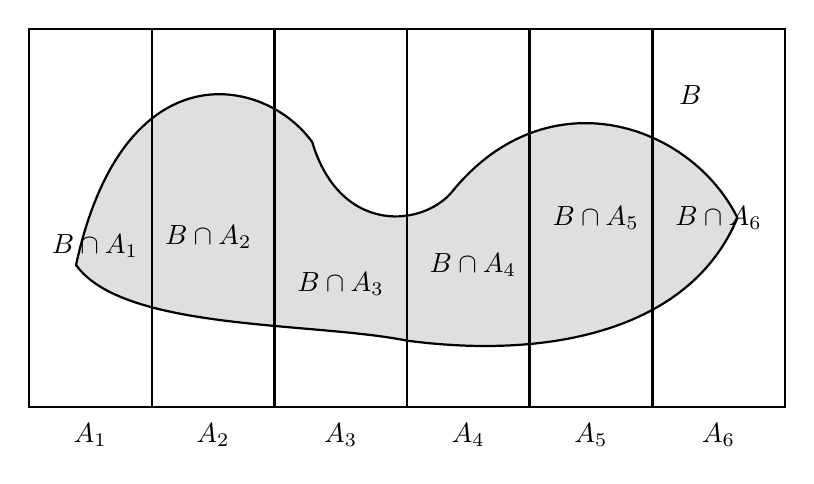
\begin{tikzpicture}[scale=1.2]

% Draw the sample space rectangle
\draw[thick] (0,0) rectangle (8,4);

% Label Ai regions
\node at (0.65,-0.3) {$A_1$};
\node at (1.95,-0.3) {$A_2$};
\node at (3.3,-0.3) {$A_3$};
\node at (4.65,-0.3) {$A_4$};
\node at (5.95,-0.3) {$A_5$};
\node at (7.3,-0.3) {$A_6$};

% Draw event B as an irregular shaded region
\filldraw[fill=gray!25, draw=black, line join=round, thick]
  (0.5,1.5) .. controls (1,3.8) and (2.5,3.5) .. (3,2.8)
  .. controls (3.3,1.8) and (4.2,1.9) .. (4.5,2.3)
  .. controls (5.5,3.5) and (7,3) .. (7.5,2)
  .. controls (7,0.8) and (5.5,0.5) .. (4,0.7)
  .. controls (3,0.9) and (1,0.8) .. (0.5,1.5) -- cycle;

% Draw partitions A1 to A6
\foreach \x in {0,1.3,2.6,4,5.3,6.6,8}
  \draw[thick] (\x,0) -- (\x,4);

% Label B region
\node at (7,3.3) {$B$};

% Label intersections B ∩ Ai
\node at (0.7,1.7) {$B\cap A_1$};
\node at (1.9,1.8) {$B\cap A_2$};
\node at (3.3,1.3) {$B\cap A_3$};
\node at (4.7,1.5) {$B\cap A_4$};
\node at (6.0,2.0) {$B\cap A_5$};
\node at (7.3,2.0) {$B\cap A_6$};

\end{tikzpicture}
\end{center}
}

\example{
A patient named Fred is tested for a
disease called conditionitis, a medical condition that afflicts 1\% of the population. The test result is positive, i.e., the test claims that Fred has the disease. Let D be the event that Fred has the disease and T be the event that he tests positive.

Suppose that the test is “95\% accurate”; there are different measures of the accuracy of a test, but in this problem it is assumed to mean that $P(T|D) = 0.95$ and $P(T^c|D^c) = 0.95$. The quantity $P(T|D)$ is known as the \textit{sensitivity} or \textit{true positive rate} of the test, and $P(T^c|D^c)$ is known as the \textit{specificity} or \textit{true negative rate}.

Find the conditional probability that Fred has conditionitis, given the evidence provided by the test result.

\textit{Solution:} Applying Bayes’ rule and the law of total probability, we have
\begin{align*}
    P(D|T) &= \frac{P(T|D)P(D)}{P(T)}\\
    &= \frac{P(T|D)P(D)}{P(T|D)P(D) + P(T|D^c)P(D^c)}\\
    &\approx 0.16
\end{align*}
}

\theorem{\textbf{Bayes’ rule with extra conditioning} (\bookref{Ch. 2.4})\\
Provided that $P(A \cap E) > 0$ and $P(B \cap E) > 0$, we have
$$
P(A|B, E) = \frac{P(B|A, E)P(A|E)}{P(B|E)}.
$$
}

\theorem{\textbf{LOTP with extra conditioning} (\bookref{Ch. 2.4})\\
Let $A_1, \dots, A_n$ be a partition of $S$. Provided that $P(A_i \cap E) > 0$ for all $i$, we have
$$
P(B|E) = \sum^n_{i=1} P(B|A_i, E) P(A_i|E).
$$
}

The extra conditioning forms of Bayes’ rule and LOTP can be proved similarly to how we verified that $\tilde{P}(A) = P(A|E)$ satisfies the axioms of probability, but they also follow directly from the “metatheorem” that \textit{conditional probabilities are probabilities}.
\newpage
\lecture{6: Monty Hall, Simpson's Paradox}
\textbf{Key Topics:} Monty Hall, Simpson's Paradox

\subsection*{Lecture Summary}
\begin{itemize}
    \item Monty Hall
    \item Simpson's Paradox
\end{itemize}

\subsection*{Monty Hall}
On the game show Let’s Make a Deal, hosted by Monty Hall, a contestant chooses one of three closed doors, two of which have a goat behind them and one of which has a car. Monty, who knows where the car is, then opens one of the two remaining doors. The door he opens always has a goat behind it (he never reveals the car!). If he has a choice, then he picks a door at random with equal probabilities. Monty then offers the contestant the option of switching to the other unopened door. If the contestant’s goal is to get the car, should she switch doors?
\begin{figure}[ht]
    \centering
    \includegraphics[width=0.5\textwidth]{lectures/images/lect_06_doors.png}
\end{figure}\\
\noindent
\textit{Solution:}

Let’s label the doors 1 through 3. Without loss of generality, we can assume the contestant picked door 1 (if she didn’t pick door 1, we could simply relabel the doors, or rewrite this solution with the door numbers permuted). Monty opens a door, revealing a goat. As the contestant decides whether or not to switch to the remaining unopened door, what does she really wish she knew? Naturally, her decision would be a lot easier if she knew where the car was! This suggests that we should condition on the location of the car. Let $C_i$ be the event that the car is behind door $i$, for $i = 1, 2, 3$. By the law of total probability,
$$
P(\text{get car}) = P(\text{get car}|C_1)\cdot \frac{1}{3} + P(\text{get car}|C_2)\cdot \frac{1}{3} + P(\text{get car}|C_3)\cdot \frac{1}{3}.
$$

Suppose the contestant employs the switching strategy. If the car is behind door 1, then switching will fail, so $P(\text{get car}|C_1) = 0$. If the car is behind door 2 or 3, then because Monty always reveals a goat, the remaining unopened door must contain the car, so switching will succeed. Thus,
$$
P(\text{get car}) = 0 \cdot \frac{1}{3} + 1\cdot \frac{1}{3} + 1\cdot \frac{1}{3} = \frac{2}{3},
$$
so the switching strategy succeeds 2/3 of the time. The contestant should switch to the other door.

There’s a subtlety though, which is that when the contestant chooses whether to switch, she also knows which door Monty opened. We showed that the unconditional probability of success is 2/3 (when following the switching strategy), but let’s also show that the conditional probability of success for switching, given the information that Monty provides, is also 2/3.

Let $M_j$ be the event that Monty opens door $j$, for $j = 2, 3$. Then
$$
P(\text{get car}) = P(\text{get car}|M_2)P(M_2) + P(\text{get car}|M_3)P(M_3),
$$
where by symmetry $P(M_2) = P(M_3) = 1/2$ and $P(\text{get car}|M_2) = P(\text{get car}|M_3)$. The symmetry here is that there is nothing in the statement of the problem that distinguishes between door 2 and door 3; in contrast, to the Lazy Monty Hall which considers a scenario where Monty enjoys opening door 2 more than he enjoys opening door 3.

Let $x = P(\text{get car}|M_2) = P(\text{get car}|M_3)$. Plugging in what we know,
$$
\frac{2}{3} = P(\text{get car}) = \frac{x}{2} + \frac{x}{2} = x,
$$
as claimed.

Bayes’ rule also works nicely for finding the conditional probability of success using the switching strategy, given the evidence. Suppose that Monty opens door 2. Using the notation and results above,
$$
P(C_1|M_2) = \frac{P(M_2|C_1)P(C_1)}{P(M_2)} = \frac{(1/2)(1/3)}{1/2} = \frac{1}{3}.
$$

So given that Monty opens door 2, there is a 1/3 chance that the contestant’s original choice of door has the car, which means that there is a 2/3 chance that the switching strategy will succeed.

Many people, upon seeing this problem for the first time, argue that there is no advantage to switching: “There are two doors remaining, and one of them has the car, so the chances are 50-50.” After the last chapter, we recognize that this argument misapplies the naive definition of probability. Yet the naive definition, even when inappropriate, has a powerful hold on people’s intuitions.

\subsection*{Simpson's Paradox}
Two doctors, Dr. Hibbert and Dr. Nick, each perform two types of surgeries: heart surgery and Band-Aid removal. Each surgery can be either a success or a failure. The two doctors’ respective records are given in the following tables.\\

\begin{minipage}{0.45\linewidth}
\centering
\begin{tabular}{lcc}
\toprule
 & Heart & Band-Aid \\
\midrule
Success & 70 & 10 \\
Failure & 20 & 0 \\
\bottomrule
\end{tabular}

\vspace{2mm}
Dr. Hibbert
\end{minipage}
\hfill
\begin{minipage}{0.45\linewidth}
\centering
\begin{tabular}{lcc}
\toprule
 & Heart & Band-Aid \\
\midrule
Success & 2 & 81 \\
Failure & 8 & 9 \\
\bottomrule
\end{tabular}

\vspace{2mm}
Dr. Nick
\end{minipage}\\

Dr. Hibbert had a higher success rate than Dr. Nick in heart surgeries: 70 out of 90 versus 2 out of 10. Dr. Hibbert also had a higher success rate in Band-Aid removal: 10 out of 10 versus 81 out of 90. But if we aggregate across the two types of surgeries to compare overall surgery success rates, Dr. Hibbert was successful in 80 out of 100 surgeries while Dr. Nick was successful in 83 out of 100 surgeries: Dr. Nick’s overall success rate is higher!

What’s happening is that Dr. Hibbert, presumably due to his reputation as the superior doctor, is performing a greater number of heart surgeries, which are inherently riskier than Band-Aid removals. His overall success rate is lower not because of lesser skill on any particular type of surgery, but because a larger fraction of his surgeries are risky.

Let’s use event notation to make this precise. For events $A$, $B$, and $C$, we say that we have a \textit{Simpson’s paradox} if
\begin{align*}
    P(A|B, C) &< P(A|B^c, C)\\
    P(A|B, C^c) &< P(A|B^c, C^c),
\end{align*}
but
$$
P(A|B) > P(A|B^c).
$$

In this case, let $A$ be the event of a successful surgery, $B$ be the event that Dr. Nick is the surgeon, and $C$ be the event that the surgery is a heart surgery. The conditions for Simpson’s paradox are fulfilled because the probability of a successful surgery is lower under Dr. Nick than under Dr. Hibbert whether we condition on heart surgery or on Band-Aid removal, but the overall probability of success is higher for Dr. Nick.

The law of total probability tells us mathematically why this can happen:
\begin{align*}
    P(A|B) &= P(A|C, B)P(C|B) + P(A|C^c, B)P(C^c|B)\\
    P(A|B^c) &= P(A|C, B^c)P(C|B^c) + P(A|C^c, B^c)P(C^c|B^c).
\end{align*}

The above equations express $P(A|B)$ as a weighted average of $P(A|C, B)$ and $P(A|C^c, B)$, and $P(A|B^c)$ as a weighted average of $P(A|C, B^c)$ and $P(A|C^c, B^c)$. If the corresponding weights were the same in both of these weighted averages, then Simpson’s paradox could not occur. But the weights here are \textit{different}:
$$
P(C|B) < P(C|B^c) \text{ and } P(C^c|B) > P(C^c|B^c),
$$
since Dr. Nick is much less likely than Dr. Hibbert to be performing a heart surgery.

Although we have
$$
P(A|C, B) < P(A|C, B^c)
$$
and
$$
P(A|C^c, B) < P(A|C^c, B^c),
$$
the fact that the weights are so different results in the inequality flipping when we do not condition on whether or not $C$ occurred:
$$
P(A|B) > P(A|B^c).
$$

Numerically, the two weighted averages are
\begin{align*}
    P(A|B) &= 0.83 = (2/10) \cdot 0.1 + (81/90) \cdot 0.9\\
    P(A|B^c) &= 0.80 = (70/90) \cdot 0.9 + (10/10) \cdot 0.1.
\end{align*}

The first equation (corresponding to Dr. Nick) puts much more weight on the second term (corresponding to the easier surgery) than does the second equation.

Aggregation across different types of surgeries presents a misleading picture of the doctors’ abilities because we lose the information about which doctor tends to perform which type of surgery. When we think \textit{confounding variables} like surgery type could be at play, we should examine the disaggregated data to see what is really going on.
\newpage
\lecture{7: Gambler's Ruin and Random Variables}
\textbf{Key Topics:} Gambler's Ruin, Random Variable

\subsection*{Lecture Summary}
\begin{itemize}
    \item Gambler's Ruin
    \item Random Variable definition and examples
\end{itemize}

\subsection*{Core Concepts}
\definition{\textbf{Random variable} (\bookref{Ch. 3.1})\\
Given an experiment with sample space $S$, a \textit{random variable} (r.v.) is a function from the sample space $S$ to the real numbers $\mathbb{R}$. It is common, but not required, to denote random variables by capital letters.\\

Thus, a random variable $X$ assigns a numerical value $X(s)$ to each possible outcome $s$ of the experiment. The randomness comes from the fact that we have a random experiment (with probabilities described by the probability function $P$); the mapping itself is deterministic.
}

\subsection*{Gambler's Ruin}
Two gamblers, A and B, make a sequence of \$1 bets. In each bet, gambler A has probability $p$ of winning, and gambler B has probability $q = 1 - p$ of winning. Gambler A starts with $i$ dollars and gambler B starts with $N - i$ dollars; the total wealth between the two remains constant since every time A loses a dollar, the dollar goes to B, and vice versa.

We can visualize this game as a \textit{random walk} on the integers between 0 and $N$, where $p$ is the probability of going to the right in a given step: imagine a person who starts at position $i$ and, at each time step, moves one step to the right with
probability $p$ and one step to the left with probability $q = 1 - p$. The game ends when either A or B is ruined, i.e., when the random walk reaches 0 or $N$. What is the probability that A wins the game (walking away with all the money)?\\

\textit{Solution:}

We recognize that this game has a recursive structure: after the first step, it’s exactly the same game, except that A’s wealth is now either $i + 1$ or $i - 1$. Let $p_i$ be the probability that A wins the game, given that A starts with $i$ dollars. We will use first-step analysis to solve for the $p_i$. Let $W$ be the event that A wins the game. By LOTP, conditioning on the outcome of the first round, we have
\begin{align*}
    p_i &= P(W|\text{A starts at $i$, wins round 1}) \cdot p + P(W|\text{A starts at $i$, loses round 1}) \cdot q \\
    &= P(W|\text{A starts at $i+1$}) \cdot p + P(W|\text{A starts at $i-1$}) \cdot q\\
    &= p_{i+1} \cdot p + p_{i-1} \cdot q
\end{align*}

This must be true for all $i$ from 1 to $N - 1$, and we also have the boundary conditions $p_0 = 0$ and $p_N = 1$. Now we can solve this equation, called a \textit{difference equation}, to obtain the $p_i$.

The characteristic equation of the difference equation is $px^2 - x + q = 0$, which has roots 1 and $q/p$. If $p \ne q$, these roots are distinct, and the general solution is
$$
p_i = A \cdot 1^i + B \cdot \left( \frac{q}{p}\right)^i.
$$
Using the boundary conditions $p_0 = 0$ and $p_N = 1$, we get
$$
    p_i =
    \begin{cases}
        \frac{1 - \left( \frac{q}{p} \right) ^i}{1 - \left( \frac{p}{q} \right) ^N} & \text{if } p \ne q\\
        \frac{i}{N} & \text{if } p = q 
    \end{cases}
$$

\subsection*{Random Variables}
Let’s consider a coin-tossing example. The structure of the problem is that we have a sequence of trials where there are two possible outcomes for each trial. Here we think of the possible outcomes as $H$ (Heads) and $T$ (Tails), but we could just as well think of them as “success” and “failure” or as 1 and 0, for example.

\example{\textbf{Coin tosses}\\
Consider an experiment where we toss a fair coin twice. The sample space consists of four possible outcomes: $S = \{HH, HT, TH, TT$\}. Here are some random variables on this space (for practice, you can think up some of your own). Each r.v. is a numerical summary of some
aspect of the experiment.
\begin{itemize}
    \item Let $X$ be the number of Heads. This is a random variable with possible values 0, 1, and 2. Viewed as a function, $X$ assigns the value 2 to the outcome $HH$, 1 to the outcomes $HT$ and $TH$, and 0 to the outcome $TT$. That is,
    $$
    X(HH) = 2, X(HT) = X(TH) = 1, X(TT) = 0.
    $$

    \item Let $Y$ be the number of Tails. In terms of $X$, we have $Y =  2 - X$. In other words, $Y$ and $2 - X$ are the same r.v.: $Y(s) = 2 - X(s)$ for all $s$.

    \item Let $I$ be 1 if the first toss lands Heads and 0 otherwise. Then $I$ assigns the value 1 to the outcomes $HH$ and $HT$ and 0 to the outcomes $TH$ and $TT$. This r.v. is an example of what is called an indicator random variable since it indicates whether the first toss lands Heads, using 1 to mean “yes” and 0 to mean “no”.
\end{itemize}

We can also encode the sample space as $\{(1, 1),(1, 0),(0, 1),(0, 0)\}$, where 1 is the code for Heads and 0 is the code for Tails. Then we can give explicit formulas for $X$, $Y$, $I$:
$$
X(s1, s2) = s1 + s2\text{, } Y (s1, s2) = 2 - s1 - s2\text{,  } I(s1, s2) = s1,
$$
where for simplicity we write X(s1, s2) to mean X((s1, s2)), etc.
}

For most r.v.s we will consider, it is tedious or infeasible to write down an explicit formula in this way. Fortunately, it is usually unnecessary to do so, since (as we saw in this example) there are other ways to define an r.v., and (as we will see
throughout the rest of this book) there are many ways to study the properties of an r.v. other than by doing computations with an explicit formula for what it maps each outcome $s$ to.
\newpage
\lecture{8: Random Variables and Their Distributions}
\textbf{Key Topics:} Gambler's Ruin, Random Variable

\subsection*{Lecture Summary}
\begin{itemize}
    \item Gambler's Ruin
    \item Random Variable definition and examples
\end{itemize}

\subsection*{Core Concepts}
\definition{\textbf{Discrete random variable} (\bookref{Ch. 3.2})\\
A random variable $X$ is said to be \textit{discrete} if there is a finite list of values $a_1, a_2, \dots , a_n$ or an infinite list of values $a_1, a_2, \dots$ such that $P(X = a_j \text{ for some $j$}) = P(X\ \in \{a_1, a_2, \dots\}) = 1$. If $X$ is a discrete r.v., then the finite or countably infinite set of values $x$ such that $P(X = x) > 0$ is called the \textit{support} of $X$.
}

\definition{\textbf{Probability mass function} (\bookref{Ch. 3.2})\\
The \textit{probability mass function} (PMF) of a discrete r.v. $X$ is the function $p_X$ given by $p_X(x) = P(X = x)$. Note that this is positive if $x$ is in the support of $X$, and 0 otherwise.
}

\note{
In writing $P(X = x)$, we are using $X = x$ to denote an event, consisting of all outcomes $s$ to which $X$ assigns the number $x$. This event is also written as $\{X = x\}$; formally, $\{X = x\}$ is defined as $\{s \in S \colon X(s) = x\}$, but writing $\{X = x\}$ is shorter and more intuitive. Going back to the 'Coin toss' example, if $X$ is the number of Heads in two fair coin tosses, then $\{X = 1\}$ consists of the sample outcomes $HT$ and $TH$, which are the two outcomes to which $X$ assigns the number 1. Since $\{HT, TH\}$ is a subset of the sample space, it is an event. So it makes sense to talk about $P(X = 1)$, or more generally, $P(X = x)$. If $\{X = x\}$ were anything other than an event, it would make no sense to calculate its probability! It does not make sense to write “$P(X)$”; we can only take the probability of an event, not of an r.v.
}

\theorem{\textbf{Valid PMFs} (\bookref{Ch. 3.2})\\
Let $X$ be a discrete r.v. with support $x_1, x_2, \dots$ (assume these values are distinct and, for notational simplicity, that the support is countably infinite; the analogous results hold if the support is finite). The PMF $p_X$ of $X$ must satisfy the following two criteria:
\begin{itemize}
    \item Nonnegative: $p_X(x) > 0$ if $x = x_j$ for some $j$, and $p_X(x) = 0$ otherwise;
    \item Sums to 1: $\sum_j p_X(x_j) = 1$.
\end{itemize}
}

\definition{\textbf{Cumulative distribution function} (\bookref{Ch. 3.6})\\
The \textit{cumulative distribution function} (CDF) of an r.v. X is the function $F_X$ given by $F_X(x) = P(X \le x)$. When there is no risk of ambiguity, we sometimes drop the subscript and just write F (or some other letter) for a CDF.
}

\subsection*{Bernoulli and Binomial}
\definition{\textbf{Bernoulli distribution} (\bookref{Ch. 3.3})\\
An r.v. $X$ is said to have the \textit{Bernoulli distribution} with parameter $p$ if
$$
P(X = 1) = p \quad \text{and} \quad P(X = 0) = 1 - p, \quad\text{where } 0 < p < 1
$$
We write this as $X \sim \Bern(p)$. The symbol $\sim$ is read “is distributed as”.
}

\definition{\textbf{Indicator random variable} (\bookref{Ch. 3.3})\\
The \textit{indicator random variable} of an event $A$ is the r.v. which equals 1 if $A$ occurs and 0 otherwise. We will denote the indicator r.v. of $A$ by $I_A$ or $I(A)$. Note that $I_A \sim \Bern(p)$ with $p = P(A)$.
}

\story{\textbf{Bernoulli trial}\\
An experiment that can result in either a “success” or a “failure” (but not both) is called a \textit{Bernoulli trial}. A Bernoulli random variable can be thought of as the \textit{indicator of success} in a Bernoulli trial: it equals 1 if success occurs and 0 if failure occurs in the trial.
}

Because of this story, the parameter $p$ is often called the \textit{success probability} of the $\Bern(p)$ distribution. Once we start thinking about Bernoulli trials, it’s hard not to start thinking about what happens when we have more than one trial.

\story{\textbf{Binomial distribution}\\
Suppose that $n$ independent Bernoulli trials are performed, each with the same success probability $p$. Let $X$ be the number of successes. The distribution of $X$ is called the \textit{Binomial distribution} with parameters $n$ and $p$. We write $X \sim \Bin(n, p)$ to mean that $X$ has the Binomial distribution with parameters $n$ and $p$, where $n$ is a positive integer and $0 < p < 1$.
}

Notice that we define the Binomial distribution not by its PMF, but by a \textit{story} about the type of experiment that could give rise to a random variable with a Binomial distribution. The most famous distributions in statistics all have stories which explain why they are so often used as models for data, or as the building blocks for more complicated distributions.

Thinking about the named distributions first and foremost in terms of their stories has many benefits. It facilitates pattern recognition, allowing us to see when two problems are essentially identical in structure; it often leads to cleaner solutions that avoid PMF calculations altogether; and it helps us understand how the named distributions are connected to one another. Here it is clear that $\Bern(p)$ is the same distribution as $\Bin(1, p)$: the Bernoulli is a special case of the Binomial.

Using the story definition of the Binomial, let’s find its PMF:

\theorem{\textbf{Binomial PMF} (\bookref{Ch. 3.3})\\
If $X \sim \Bin(n, p)$, then the PMF of $X$ is
$$
P(X=k) = \binom{n}{k} p^k (1-p)^{n-k}
$$
for $k = 0, 1, \dots , n$ (and $P(X = k) = 0$ otherwise).\\

\textit{Proof:}\\
An experiment consisting of $n$ independent Bernoulli trials produces a sequence of successes and failures. The probability of any specific sequence of $k$ successes and $n - k$ failures is $p^k (1 - p)^{n-k}$. There are $\binom{n}{k}$ such sequences, since we
just need to select where the successes are. Therefore, letting $X$ be the number of successes,
$$
P(X=k) = \binom{n}{k} p^k (1-p)^{n-k}
$$
for $k = 0, 1, \dots , n$, and $P(X = k) = 0$ otherwise. This is a valid PMF because it is nonnegative and it sums to 1 by the binomial theorem.
}

\note{
To save writing, it is often left implicit that a PMF is zero wherever it is not specified to be nonzero, but in any case it is important to understand what the support of a random variable is, and good practice to check that PMFs are valid. If two discrete r.v.s have the same PMF, then they also must have the same support.
So we sometimes refer to the support of a discrete \textit{distribution}; this is the support of any r.v. with that distribution.
}

\theorem{\textbf{Sum of indicator r.v.s} (\bookref{Ch. 3.8})\\
If $X \sim \Bin(n, p)$, viewed as the number of successes in $n$ independent Bernoulli trials with success probability $p$, then we can write $X = X_1+ \cdots +X_n$ where the $X_i$ are i.i.d. $\Bern(p)$ (i.i.d. stands for independent, identically distributed).
}

\theorem{\textbf{Sum of two binomials} (\bookref{Ch. 3.8})\\
If $X \sim \Bin(n, p)$, $Y \sim \Bin(m, p)$, and $X$ is independent of $Y$, then $X + Y \sim \Bin(n + m, p)$.\\

\textit{Proof.} We present three proofs, since each illustrates a useful technique.\\
1. Story: By the Binomial story, $X$ is the number of successes in $n$ independent trials and $Y$ is the number of successes in $m$ additional independent trials, all with the same success probability, so $X + Y$ is the total number of successes in the $n + m$ trials, which is the story of the $\Bin(n + m, p)$ distribution.\\

2. Representation: A much simpler proof is to represent both $X$ and $Y$ as the sum of i.i.d. $\Bern(p)$ r.v.s: $X = X_1 + \cdots + X_n$ and $Y = Y_1 + \cdots + Y_m$, where the $X_i$ and $Y_j$ are all i.i.d. $\Bern(p)$. Then $X + Y$ is the sum of $n + m$ i.i.d. $\Bern(p)$ r.v.s, so its distribution, by the previous theorem, is $\Bin(n + m, p)$.

3. LOTP: We can directly find the PMF of $X + Y$ by conditioning on $X$ (or $Y$, whichever we prefer) and using the law of total probability:
\begin{align*}
    P(X+Y=k) &= \sum^k_{j=0} P(X+Y=k | X=j)P(X=j)\\
    &= \sum^k_{j=0} P(Y=k-j)P(X=j)\\
    &= \sum^k_{j=0} \binom{m}{k-j}p^mq^{m-k+j}\binom{n}{j}p^jq^{n-j}\\
    &= p^k q^{n+m-k} \sum^k_{j=0} \binom{m}{k-j} \binom{n}{j}\\
    &= \binom{n+m}{k}p^k q^{n+m-k}
\end{align*}
In the second line, we used the independence of X and Y to justify dropping the conditioning. In the last line, we used Vermonde's identity.
}

\subsection*{Hypergeometric}
If we have an urn filled with $w$ white and $b$ black balls, then drawing $n$ balls out of the urn with replacement yields a $\Bin(n, w/(w + b))$ distribution for the number of white balls obtained in $n$ trials, since the draws are independent Bernoulli trials, each with probability $w/(w+b)$ of success. If we instead sample \textit{without replacement}, then the number of white balls follows a \textit{Hypergeometric distribution}.

\story{\textbf{Hypergeometric distribution}\\
Consider an urn with $w$ white balls and $b$ black balls. We draw $n$ balls out of the urn at random without replacement, such that all $\binom{w+b}{n}$ samples are equally likely. Let $X$ be the number of white balls in the sample. Then $X$ is said to have the \textit{Hypergeometric distribution} with parameters $w$, $b$, and n  $n$; we denote this by $X \sim \HGeom(w, b, n)$.
}

\theorem{\textbf{Hypergeometric PMF} (\bookref{Ch. 3.4})\\
If $X \sim \HGeom(w, b, n)$, then the PMF of $X$ is
$$
P(X=k) = \frac{\binom{w}{k} \binom{b}{n-k}}{\binom{w+b}{n}},
$$.
for integers $k$ satisfying $0 \le k \le w$ and $0 \le n-k \le b$, and $P(X = k) = 0$ otherwise.\\

\textit{Proof:}\\
To get $P(X = k)$, we first count the number of possible ways to draw exactly $k$ white balls and $n - k$ black balls from the urn (without distinguishing between different orderings for getting the same set of balls). If $k > w$ or $n - k > b$, then the draw is impossible. Otherwise, there are $\binom{w}{k} \binom{b}{n-k}$ ways to draw $k$ white and $n - k$ black balls by the multiplication rule, and there are $\binom{w+b}{n}$ total ways to draw $n$ balls. Since all samples are equally likely, the naive definition of probability gives
$$
P(X=k) = \frac{\binom{w}{k} \binom{b}{n-k}}{\binom{w+b}{n}}
$$
for integers $k$ satisfying $0 \le k \le w$ and $0 \le n-k \le b$. This PMF is valid because the numerator, summed over all $k$, equals $\binom{w+b}{n}$ by Vandermonde’s identity, so the PMF sums to 1.
}
\newpage

\end{document}